\documentclass[a4paper, 12pt]{article}
\usepackage[utf8]{inputenc}
\usepackage{newpxtext, newpxmath}
\usepackage[breaklinks=true]{hyperref}
\usepackage{graphicx}
\usepackage{caption}
\usepackage[left=3cm, right=2cm, top=3cm, bottom=2cm]{geometry}
\geometry{a4paper}
\usepackage{fancyhdr}
\usepackage[brazilian]{babel}
\usepackage{siunitx}
\usepackage{float}
\pagestyle{fancy}
\renewcommand{\headrulewidth}{0pt} 
\lhead{}\chead{}\rhead{}
\lfoot{}\cfoot{\thepage}\rfoot{}
\graphicspath{{../figures/}}
\sisetup{output-decimal-marker={.}}
\usepackage{amsfonts}
\usepackage{mathtools}
\usepackage{cleveref}
\usepackage{spverbatim}
\usepackage{setspace}
\usepackage{subcaption}
\usepackage{csquotes}
\usepackage{booktabs}
\usepackage{pbox}
\setlength{\parskip}{1em}
\singlespacing

\newcommand{\empt}[2]{$#1^{\langle #2 \rangle}$}
\newcommand{\sigmoid}{\text{Sigmoid}}
\newcommand{\sen}{\text{sen}}

\usepackage{amsmath}
\usepackage{enumitem}
\usepackage{tikz}
\usetikzlibrary{shapes,arrows,fit, positioning, arrows.meta}
\usetikzlibrary{backgrounds}
\usepgflibrary{shapes.multipart}
\def\layersep{2.5cm}
\def\layersepp{5cm}	

\begin{document}
\begin{titlepage}
\newcommand{\HRule}{\rule{\linewidth}{1.5mm}}
	
\center


\includegraphics[width=0.15\textwidth]{logo-unicamp.pdf}\\[1.0cm]

\textsc{\Large Programa Institucional de Bolsas de Iniciação Científica PIBIC}\\[0.5cm]

\textsc{\large Relatório Final}\\[1.5cm]

{\Large \bfseries Predição de Séries Temporais Baseada em Redes Neurais Artificiais}\\[2.5cm]

\begin{flushleft}
Submetido à \\ Pró-Reitoria de Pesquisa da Universidade Estadual de Campinas\\[1.5cm]

Departamento de Engenharia de Computação e Automação Industrial (DCA)\\
Faculdade de Engenharia Elétrica e de Computação (FEEC)\\
Universidade Estadual de Campinas (UNICAMP)\\
CEP 13083-852, Campinas - SP\\[1.0cm]

Aluno: João Pedro de Oliveira Pagnan\\
Orientador: Prof. Levy Boccato \\[4.5cm]
\end{flushleft}	
	
Campinas, \today

\end{titlepage}

\newpage

\section{Introdução}

Depois de uma exposição sobre certos modelos preditores com redes neurais artificiais e sobre as características principais de sistemas com dinâmica caótica, apresentados no relatório parcial (seções $2.1$ e $2.2$, respectivamente), este relatório final irá expor os cenários utilizados para a análise, a metodologia utilizada, os resultados obtidos e, por fim, as conclusões desta pesquisa sobre o desempenho de redes neurais artificiais na predição de séries temporais originadas por sistemas com dinâmica caótica, além de alguns detalhes sobre as arquiteturas estudadas nesta segunda parte da pesquisa, que foram a \textit{Gated Recurrent Unit} (GRU) \cite{cho2014learning} e a \textit{Echo State Network} (ESN) \cite{jaeger2007echo}. 

A seção 2 apresenta os quatro cenários escolhidos para a análise do desempenho das redes neurais, sendo dois destes a tempo discreto e dois a tempo contínuo. No caso, os sistemas a tempo discreto foram o mapa de Hénon \cite{henon1976two} e o mapa logístico \cite{may1976simple}. Já os sistemas a tempo contínuo foram o sistema de Lorenz \cite{lorenz1963deterministic} e as equações de Mackey-Glass \cite{mackey1977oscillation}.

Já na seção 3, discutiremos os dois modelos previamente citados que foram estudados e implementados, juntamente com as redes neurais apresentadas no relatório parcial, nesta segunda parte da pesquisa. 

A seção 4 realiza uma exposição da busca em grade \cite{geron2019hands} realizada em cada modelo, expondo quais foram os parâmetros testados e os critérios definidos para o processo de busca. Além disso, a seção 4 também apresentará a metodologia utilizada para definir o número de amostras de entrada de cada modelo preditor (nesse caso, chamado de $K$), além de indicar qual foi a progressão do erro quadrático médio (EQM) em função do valor de $K$ para cada modelo nos quatro cenários.

Por fim, as seções 5 e 6 apresentam os resultados e as conclusões obtidas, respectivamente, encerrando, assim, esta pesquisa de iniciação científica.
 
\section{Cenários utilizados}

Antes de falarmos sobre os cenários utilizados na análise, vale a pena reforçarmos as características principais de sistemas com dinâmica caótica. 

Sistemas caóticos se destacam pois, apesar de serem determinísticos, apresentam dependência sensitiva em relação às condições iniciais (DSCI). Dessa forma, duas trajetórias que partem de posições relativamente próximas no espaço de estados podem evoluir de uma forma totalmente distinta devido às não-linearidades presentes que amplificam as diferenças entre essas condições iniciais \cite{fiedler1994caos}.

De forma resumida, a dinâmica caótica é marcada pela presença dos seguintes aspectos \cite{attux2001dinamica}:
\begin{enumerate}
\item Forte sensibilidade com respeito às condições iniciais;
\item A evolução temporal das variáveis de estado (parâmetros de ordem do sistema) é rápida e tem uma aparência errática;
\item Um sinal originado por um sistema caótico tem espectro de potências contínuo e de faixa larga;
\item Há uma produção de informação por parte do sistema;
\item Dão origem a atratores estranhos (estruturas topológicas que ditam a evolução temporal do fluxo de um sistema caótico) \cite{ruelle1971nature}.
\end{enumerate}

Retomados os pontos principais da dinâmica caótica, daremos continuidade à discussão apresentando os cenários escolhidos para a análise. Vale mencionar que, na simulação numérica dos quatro sistemas, foram geradas $5000$ amostras para cada série temporal. Além disso, nos sistemas multidimensionais, como o mapa de Hénon e o sistema de Lorenz, consideramos apenas a variável de estado $x$ na previsão, em ambos os casos.

\subsection{Sistema de Lorenz}

O sistema de Lorenz foi um dos sistemas dinâmicos caóticos a tempo contínuo abordados nessa pesquisa. Este sistema foi um dos primeiros grandes trabalhos envolvendo a noção de regime caótico, sendo considerado por muitos a pesquisa que inaugurou a área \cite{gleick1998chaos}.

Lorenz modela, através de três equações diferenciais, o fluxo de um fluido em um volume uniformemente aquecido na camada inferior e uniformemente resfriado na camada superior \cite{lorenz1963deterministic}:
\begin{subequations}
\begin{equation}
\frac{dx}{dt} = -\sigma \cdot (x - y)
\end{equation}
\begin{equation}
\frac{dy}{dt} = x \cdot (\rho - z) - y
\end{equation}
\begin{equation}
\frac{dz}{dt} = x \cdot y - \beta \cdot z
\end{equation}
\end{subequations}
sendo $\sigma$, $\rho$ e $\beta$ constantes reais, estando relacionadas a certas características físicas do sistema, como o número de Prandtl, o número de Rayleigh e as dimensões do volume que o fluido ocupa \cite{fiedler1994caos}.

Utilizando $\sigma = 10$, $\rho = 28$ e $\beta = 8/3$, Lorenz demonstrou que esse sistema de equações diferenciais exibe comportamento caótico, sendo que a maioria das condições iniciais $[x(0)\; y(0)\; z(0)] = [0\; 0\; 0]^T$ convergem para um atrator estranho (nesse caso, atrator de Lorenz).

A figura \ref{fig:lorenz} indica a série temporal em $x$, que foi utilizada em nossa análise, para $[x(0)\; y(0)\; z(0)]^T = [0.1\; 0\; 0]^T$, e o atrator de Lorenz para a trajetória. Para a simulação, os parâmetros do sistema foram configurados para os mesmos valores utilizados por Lorenz (exibidos no parágrafo anterior), e foi utilizado $dt = 0.01$ para resolver as equações diferenciais numericamente.
\begin{figure}[H]
     \begin{subfigure}[t]{0.35\textwidth} 
         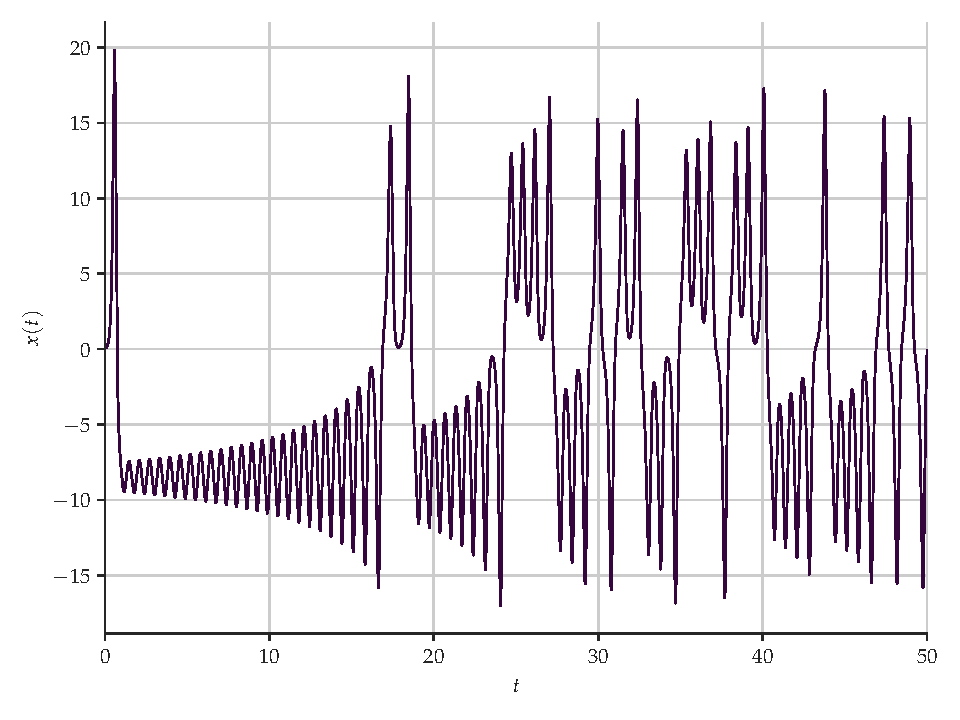
\includegraphics[scale=0.35]{serie-lorenz-x.pdf}
     \end{subfigure}
     \centering
     \begin{subfigure}[t]{0.35\textwidth}
         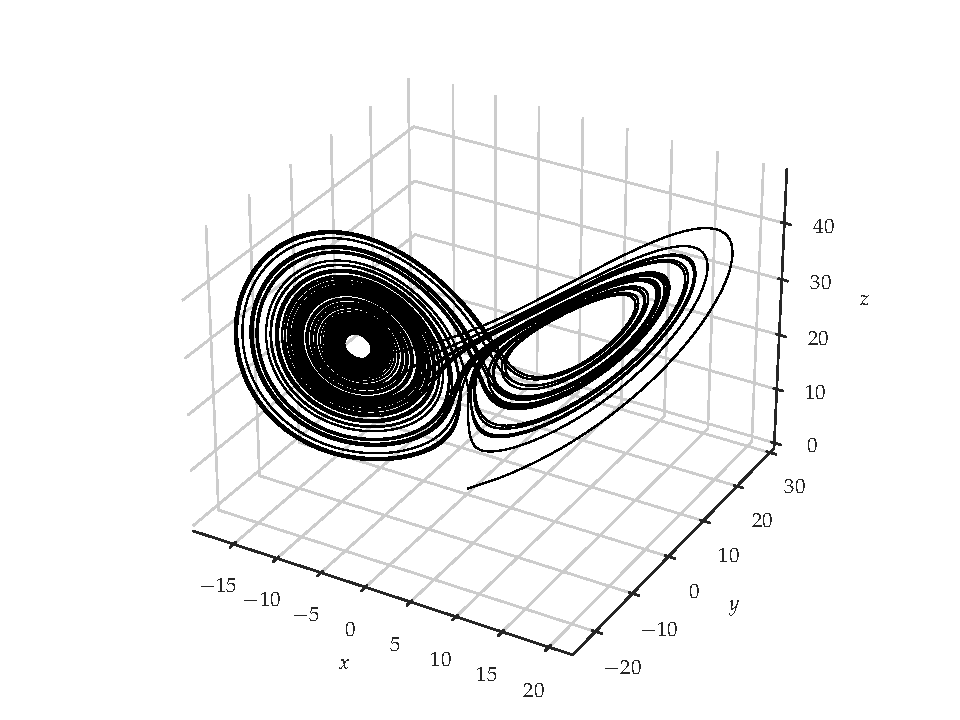
\includegraphics[scale=0.35]{diagrama-de-fases-lorenz.pdf}
     \end{subfigure}
     \caption{À esquerda, a série temporal em $x$ do sistema de Lorenz simulado e, à direita, o diagrama de fases correspondente à simulação}
     \label{fig:lorenz}
\end{figure}


\subsection{Mapa de Hénon}

O mapa de Hénon foi um dos sistemas a tempo discreto escolhidos para esta pesquisa. Esse sistema foi proposto por Michel Hénon em 1976 como um modelo simplificado de uma seção de Poincaré do atrator de Lorenz, sendo descrito pelas equações abaixo \cite{henon1976two}:
\begin{subequations}
\begin{equation}
x[n+1] = y[n] + 1 - a\cdot (x[n])^2
\end{equation}
\begin{equation}
y[n+1] = b \cdot x[n]
\end{equation}
\end{subequations}

A presença de dinâmica caótica neste sistema discreto irá depender dos valores dos parâmetros $a$ e $b$. Hénon mostrou, em sua pesquisa, que, para $a = 1.4$ e $b = 0.3$, há a presença de um atrator estranho do diagrama de fases desse sistema dinâmico discreto. 

O mapa de Hénon realiza um mapeamento de dois pontos, chamados de pontos fixos. Para os valores dos parâmetros $a$ e $b$ mencionados anteriormente, tais pontos são dados por:
$$x = \frac{\sqrt{609}-7}{28} \approx 0.631354477$$
$$y = \frac{3(\sqrt{609}-7)}{280} \approx 0.189406343$$

Um desses pontos está sobre o atrator e é instável. Tal instabilidade é confirmada quando é realizada uma análise da trajetória com outros pontos próximos a este, onde percebe-se que, dependendo da região do atrator pela qual o ponto em análise se aproxima ao ponto fixo, a trajetória irá divergir ou convergir para o ponto no atrator. 

A figura \ref{fig:henon} mostra a série temporal referente à variável $x$ e o atrator obtido com a simulação para $[x[0]\; y[0]]^T = [1\; 0]^T$.
\begin{figure}[H]
     \begin{subfigure}[t]{0.35\textwidth}
         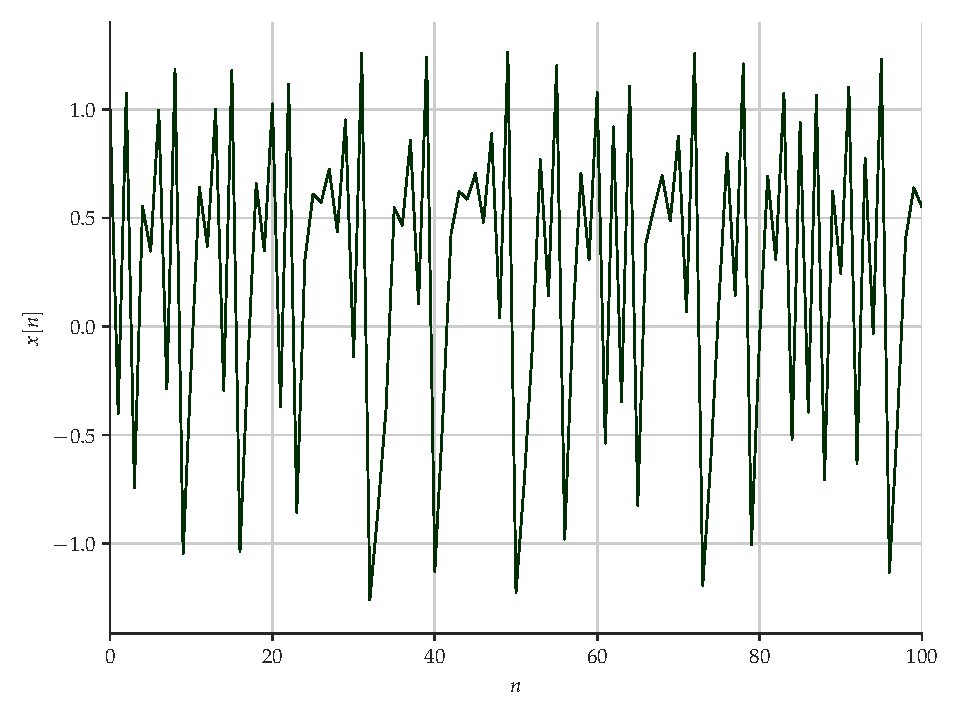
\includegraphics[scale=0.35]{serie-henon-x.pdf}
         %\caption{$y=5/x$}
     \end{subfigure}
     \centering
     \begin{subfigure}[t]{0.35\textwidth}
         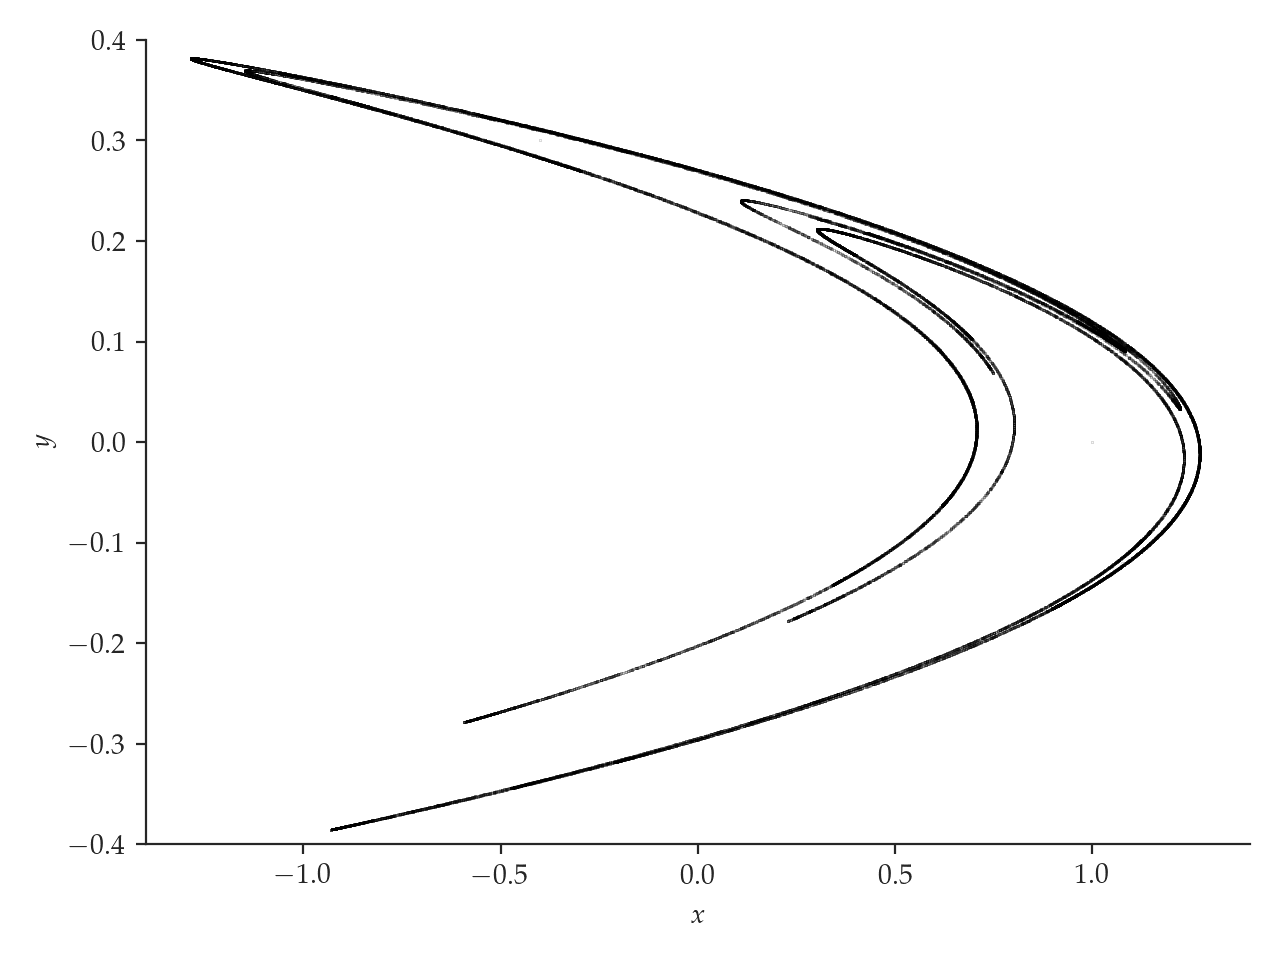
\includegraphics[scale=0.35]{mapa-de-henon.png}
         %\caption{$y=x$}
     \end{subfigure}
     \caption{À esquerda, as cem primeiras iterações da série temporal em $x$ do mapa de Hénon e, à direita, o atrator correspondente à simulação}
     \label{fig:henon}
\end{figure}

\subsection{Mapa logístico}

Descrito em 1976 por Robert May, o mapa logístico representa uma das formas de modelar a população de uma determinada espécie em certos instantes de tempo \cite{may1976simple}. A equação a diferenças que descreve esse sistema pode ser vista abaixo:
\begin{equation}\label{eq:logistic}
x[n+1] = r\cdot x[n] \cdot (1 - x[n])
\end{equation}
sendo $x_n$ um número real entre $0$ e $1$ que representa a razão entre o tamanho atual da população e o tamanho máximo desta, e tendo $r$ um valor real entre $0$ e $4$, representando a taxa de crescimento desta população.

Nesse caso, o sistema não chega a operar em caos para qualquer valor de $r$. Assim, como o estudo visa analisar o desempenho para sistemas caóticos, foi utilizado $r=3.86$, que, conforme será visto no diagrama de bifurcação abaixo, faz com que a série temporal dada pela equação (\ref{eq:logistic}) opere em caos. 

A figura \ref{fig:logistic} indica a série temporal obtida partindo de $x[0] = 0.5$ e o diagrama de bifurcação para este sistema de equações.
\begin{figure}[H]
     \begin{subfigure}[t]{0.35\textwidth} 
         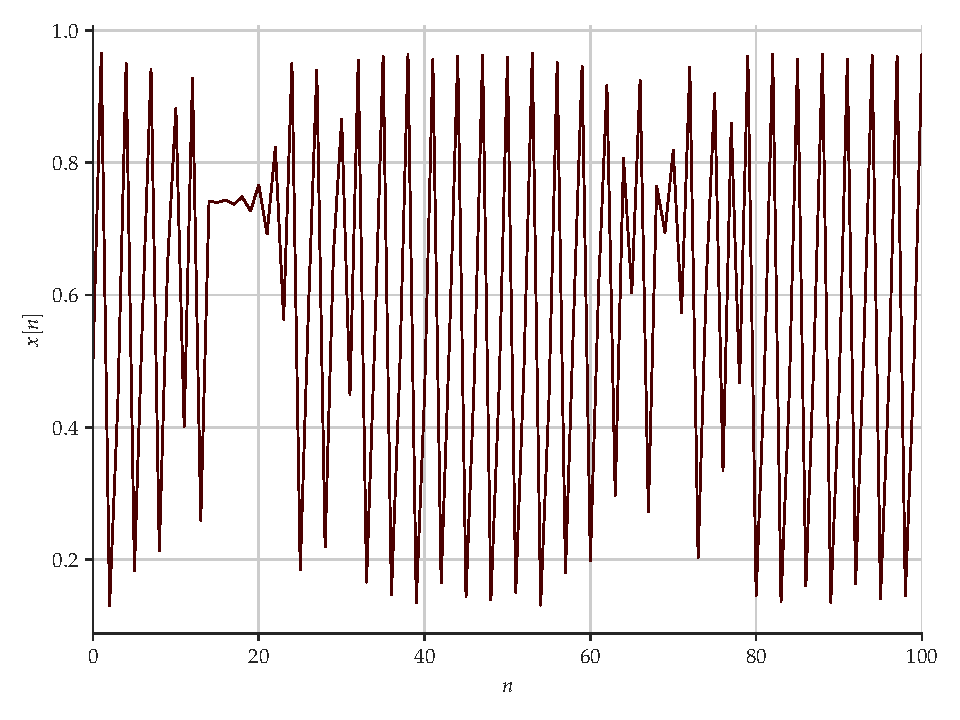
\includegraphics[scale=0.35]{serie-logistico.pdf}
         %\caption{$y=5/x$}
     \end{subfigure}
     \centering
     \begin{subfigure}[t]{0.35\textwidth} 
         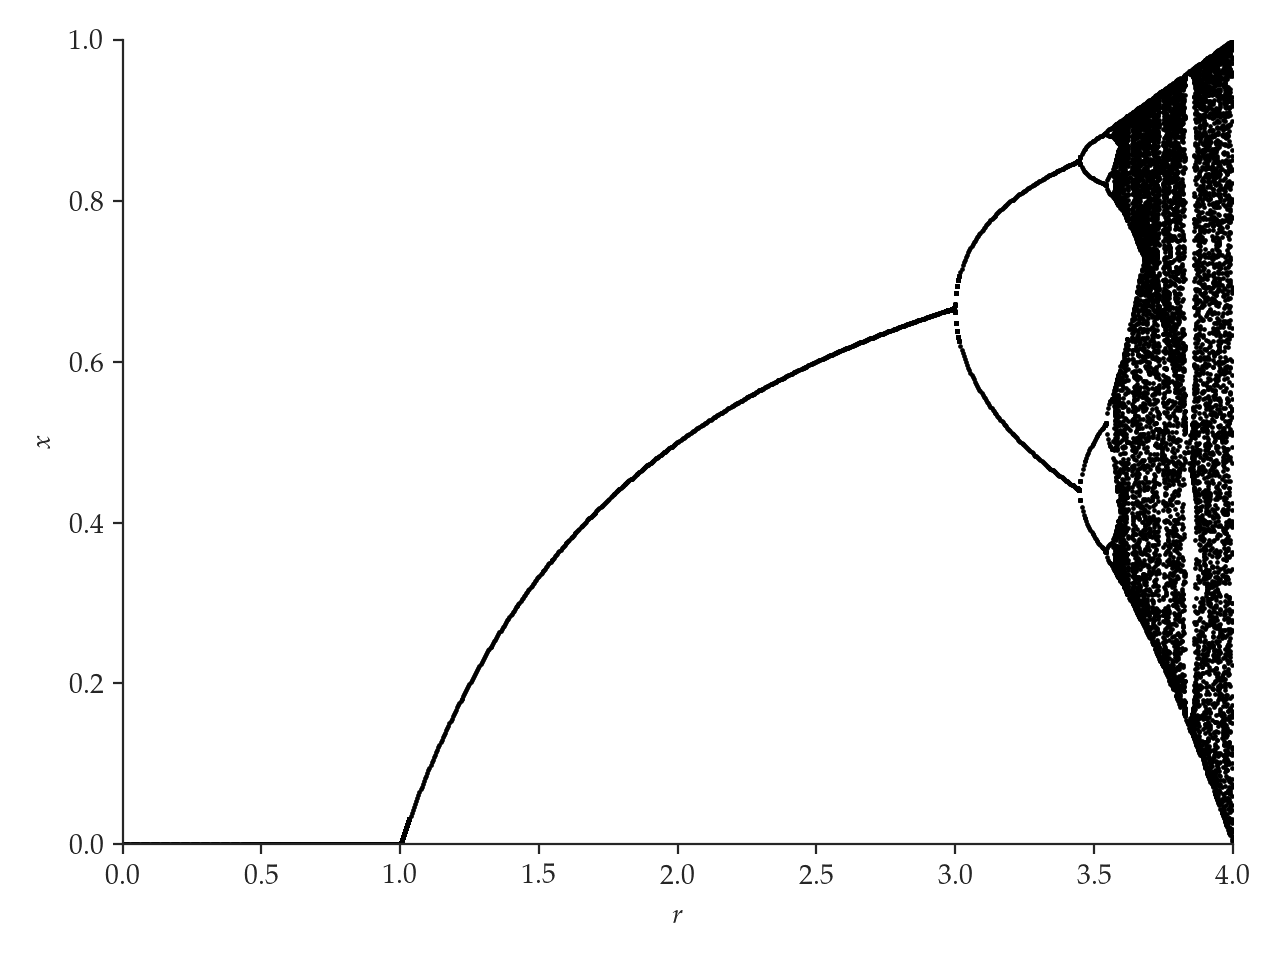
\includegraphics[scale=0.35]{mapa-logistico.png}
         %\caption{$y=x$}
     \end{subfigure}
     \caption{À esquerda, as cem primeiras iterações da série temporal do mapa logístico e, à direita, o diagrama de bifurcação deste sistema}
     \label{fig:logistic}
\end{figure}

\subsection{Equações de Mackey-Glass}

Por fim, o último sistema caótico simulado, também contínuo, está associado às equações de Mackey-Glass, as quais modelam o controle hormonal da produção de células brancas do sangue e podem ser vistas abaixo \cite{mackey1977oscillation}:
\begin{subequations}
\begin{equation}
\frac{dP(t)}{dt} = \frac{\beta_0\cdot \theta^n}{\theta^n + P(t - \tau)^n} - \gamma\cdot P(t)
\end{equation}
\begin{equation}\label{eq:mackey-glass-chaos}
\frac{dP(t)}{dt} = \frac{\beta_0\cdot \theta^n \cdot P(t - \tau)}{\theta^n + P(t - \tau)^n} - \gamma\cdot P(t)
\end{equation}
\end{subequations}
sendo $P(t)$ a densidade de tais células em um instante de tempo e $\beta_0$, $\theta$, $n$, $\tau$ e $\gamma$ valores reais relacionados a certos parâmetros hormonais de um organismo, geralmente sendo determinados experimentalmente.

Neste caso, conforme demonstrado em \cite{mackey1977oscillation}, a equação (\ref{eq:mackey-glass-chaos}) exibe comportamento caótico para valores mais altos de $\tau$. Para a simulação numérica, foi utilizado $n = 10$, $\gamma = 0.1$, $\beta = 0.2$, $\theta = 1$, $\tau = 22$, $dt = 1.0$ e $P(0^-)=0.1$, gerando novamente $5000$ amostras. A série e o atrator obtidos podem ser vistos na figura \ref{fig:mackey-glass}.
\begin{figure}[H]
     \begin{subfigure}[t]{0.35\textwidth}
         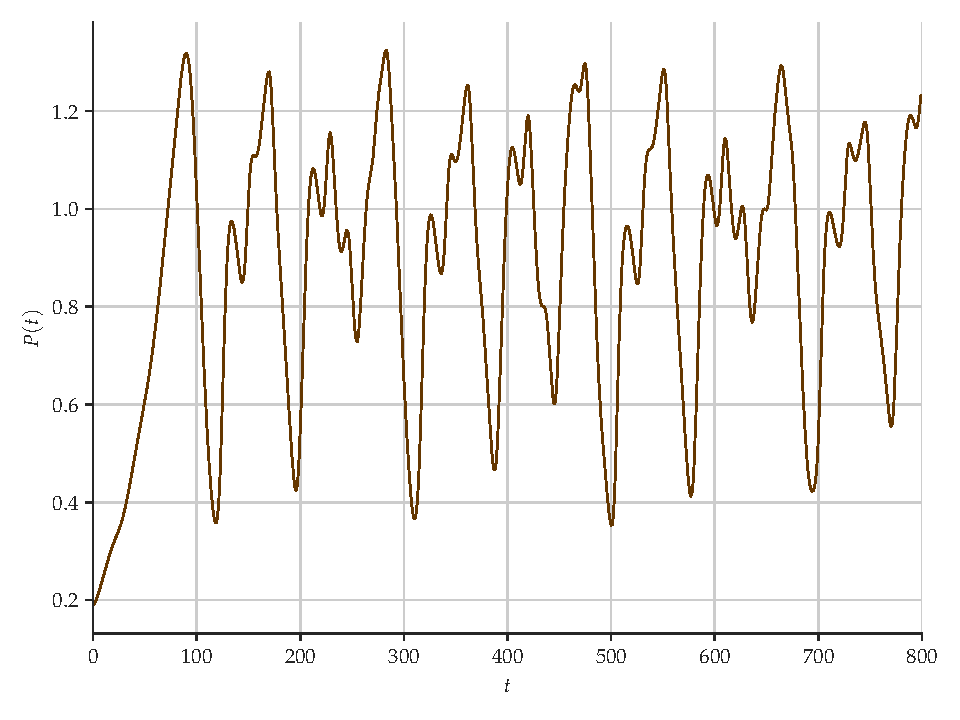
\includegraphics[scale=0.35]{serie-mackeyglass.pdf}
         %\caption{$y=5/x$}
     \end{subfigure}
     \centering
     \begin{subfigure}[t]{0.35\textwidth}
         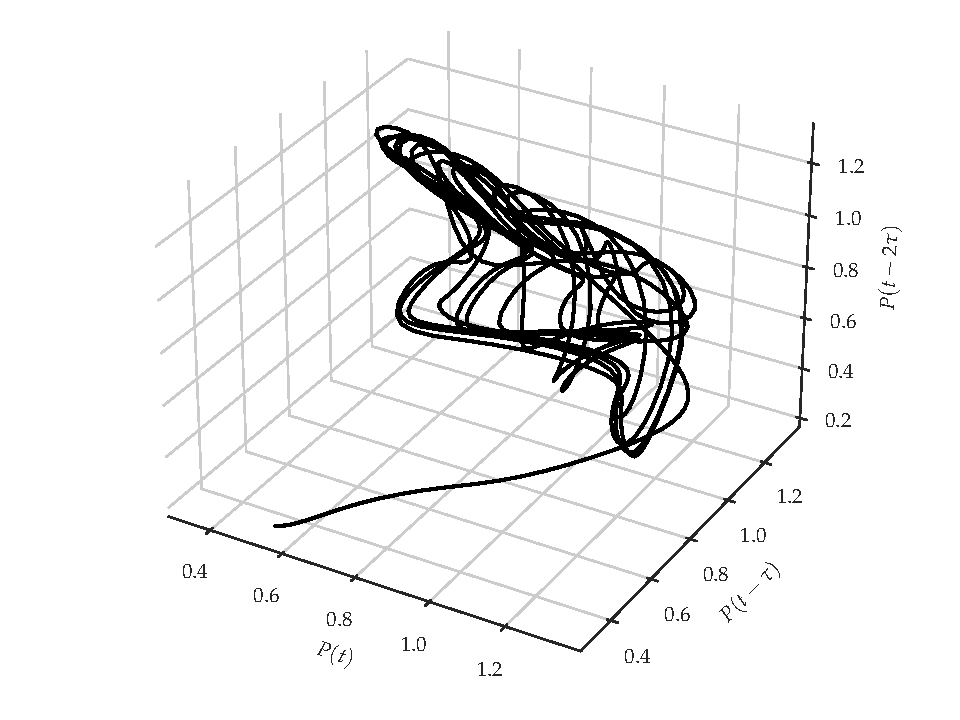
\includegraphics[scale=0.35]{atrator-mackeyglass.pdf}
         %\caption{$y=x$}
     \end{subfigure}
     \caption{À esquerda, a série temporal da equação (\ref{eq:mackey-glass-chaos}) exibida de $t = 0 $ a $t = 800$ e, à direita, o atrator correspondente à simulação}
     \label{fig:mackey-glass}
\end{figure}

Com isso, finalizamos a exposição sobre os cenários de sistemas com dinâmica caótica escolhidos para a análise comparativa. Na próxima seção, falaremos a respeito dos dois modelos estudados e implementados nesta segunda parte da pesquisa. Em seguida, apresentaremos a metodologia aplicada nesses e nos outros modelos mostrados no relatório parcial, assim como as particularidades para cada caso.

\section{Modelos avaliados}

Como o estudo de redes neurais artificiais foi iniciado na primeira metade da pesquisa, uma exposição mais detalhada dos fundamentos destes modelos (no caso, as redes MLP e as rede recorrentes LSTM) pode ser vista no relatório parcial.

Assim, as próximas duas subseções abordarão especificamente as redes recorrentes GRU e ESN.

\subsection{\textit{Gated Recurrent Unit} (GRU)}

Como já mencionamos anteriormente, as redes recorrentes \textit{Gated Recurrent Unit} possuem células computacionais semelhantes às células das redes LSTM, apresentadas no relatório parcial. Sua estrutura interna pode ser vista na figura \ref{fig:gru-cell}, juntamente com as equações que a descrevem.
\begin{figure}[H]
\begin{minipage}{0.4\textwidth}
\begin{center}
\scalebox{0.9}{
\begin{tikzpicture}[
    % GLOBAL CFG
    font=\sf \scriptsize,
    >=LaTeX,
    % Styles
    cell/.style={% For the main box
        rectangle, 
        rounded corners=5mm, 
        draw,
        very thick,
        },
    operator/.style={%For operators like +  and  x
        circle,
        draw,
        inner sep=-0.5pt,
        minimum height =.2cm,
        },
    function/.style={%For functions
        ellipse,
        draw,
        inner sep=1pt
        },
    ct/.style={% For external inputs and outputs
        circle,
        draw,
        line width = .75pt,
        minimum width=1cm,
        inner sep=1pt,
        },
    gt/.style={% For internal inputs
        rectangle,
        draw,
        minimum width=4mm,
        minimum height=3mm,
        inner sep=1pt
        },
    mylabel/.style={% something new that I have learned
        font=\tiny\sffamily
        },
    ArrowC1/.style={% Arrows with rounded corners
        rounded corners=.25cm,
        thick,
        },
    ArrowC2/.style={% Arrows with big rounded corners
        rounded corners=.5cm,
        thick,
        }
    ]

%Start drawing the thing...    
    % Draw the cell: 
    \node [cell, minimum height =4cm, minimum width=6cm] at (0,0){} ;

    % Draw inputs named ibox#
    \node [gt] (ibox1) at (-1.5,-0.75) {$\sigma$};
    \node [gt] (ibox2) at (0,-1.2) {$\sigma$};

   % Draw opérators   named mux# , add# and func#
    \node [operator] (mux1) at (-1.5,0) {$\times$};
    \node [operator] (mux2) at (0,1.5) {$\times$};
    \node [operator] (mux4) at (2.5,0.75) {$\times$};
    \node [operator] (add1) at (2.5,1.5) {+};    
    \node [function] (func1) at (2.5,0) {$\tanh$};
    \node [operator] (min1) at (1.25,0.75) {{$-1$}};

    % Draw External inputs? named as basis c,h,x
    \node[] (h) at (-4,1.5) {$\mathbf{h}(t-1)$};
    \node[] (x) at (0,-3) {$\mathbf{x}(t)$};

    % Draw External outputs? named as basis c2,h2,x2
    \node[] (h2) at (4,1.5) {$\mathbf{h}(t)$};
    \node[] (x2) at (2.5,3) {$\mathbf{y}(t)$};
    
    % Draw internals functions, named as basis fi,ii,ci,oi
    \node[] (ri) at (-1.85,-0.35) {$\mathbf{r}(t)$};
    \node[] (zi) at (0.4,-0.85) {$\mathbf{z}(t)$};  
    \node[] (gi) at (2.1,0.4) {$\mathbf{g}(t)$}; 
    
% Start connecting all.
    %Intersections and displacements are used. 
    % Drawing arrows    
    \draw [ArrowC1] (h) -- (mux2);
    \draw [->, ArrowC1] (h -| ibox1)++(-1,0) |- (ibox1);

    % Inputs

    % Internal
    \draw [->, ArrowC2] (ibox1) -- (mux1);
    
    \draw [->, ArrowC2] (ibox2) -- (mux2);
    \draw [->, ArrowC2] (mux4) -- (add1);
    \draw [->, ArrowC2] (func1) -- (mux4);
   % \draw [->, ArrowC1] (add1 -| func1)++(-0.5,0) -| (func1);

    %Outputs
    \draw [ArrowC1] (mux2) -- (add1);
    \draw [ArrowC1, ->] (add1) -- (h2);
    \draw (h2 -| x2) ++(0,-0.1) coordinate (i1);
    \draw [->, ArrowC1] (h -| mux1)++(-0.5,0) |- (mux1);
    %\draw (h -- mux1) ++(-2,2) coordinate (mux1);
    \draw [->, ArrowC2] (i1)++(0,0.2) -- (x2);
    \draw [->, ArrowC1] (x -| ibox1) ++ (+1.5,+1.25) -| (ibox1);
    \draw [->, ArrowC1] (x -| func1) ++ (-2.5,+1.25) -| (func1);
    \draw [->, ArrowC1] (x) -- (ibox2);
   % \draw [->, ArrowC1] (mux1) -- (func1);
    \draw [->, ArrowC2] (mux1 -| func1)++(-2.4,0) -- (func1) coordinate (i1);
    \draw [ArrowC1] (mux1) -- ++(+1.4,0);
    \draw [->, ArrowC1] (min1) -- (mux4);
    \draw [->, ArrowC1] (ibox2) |- (min1);

\end{tikzpicture}}
\end{center}
\end{minipage}
\; \; \; \; \; \; \;
\begin{minipage}{0.4\textwidth}
\begin{center}
{
$$$$
$$\mathbf{z}(t) = \sigma \left(\mathbf{W}_z [\mathbf{h}(t-1), \mathbf{x}(t)] + \mathbf{b}_z \right)$$
$$\mathbf{r}(t) = \sigma \left(\mathbf{W}_r [\mathbf{h}(t-1), \mathbf{x}(t)] + \mathbf{b}_r \right)$$
$$\mathbf{g}(t) = \tanh \left(\mathbf{W}_g [\mathbf{r}(t) \otimes \mathbf{h}(t-1), \mathbf{x}(t)]  + \mathbf{b}_g \right)$$
$$\mathbf{y}(t) = \mathbf{h}(t) = \mathbf{z}(t) \otimes \mathbf{h}(t-1) + (1 - \mathbf{z}(t)) \otimes \mathbf{g}(t)$$
}
\end{center}
\end{minipage}
\caption{Estrutura e equações de uma célula GRU}
\label{fig:gru-cell}
\end{figure}

Primeiramente, por ser uma rede recorrente, há uma realimentação nestas estruturas. Ou seja, a saída atual é determinada levando em conta estados passados da rede.

\subsection{\textit{Echo State Network} (ESN)}

\section{Metodologia}

\section{Resultados}

\section{Conclusão}

\bibliographystyle{ieeetr}

{\footnotesize \bibliography{bib}}

\pdfinfo{
   /Title  (Relatório EE015 - João Pedro O. Pagnan)
   /CreationDate (D:20040502195600)
}

\end{document}